\printconcepts

\exercise{In your own words, describe how to plot the polar point $P(r,\theta)$.}{Answers will vary.}

\exercise{T/F: When plotting a point with polar coordinate $P(r,\theta)$, $r$ must be positive.}{F}

\exercise{T/F: Every point in the Cartesian plane can be represented by a polar coordinate.}{T}

\exercise{T/F: Every point in the Cartesian plane can be represented uniquely by a polar coordinate.}{F}

\printproblems

\exercise{Plot the points with the given polar coordinates.\\
\begin{minipage}[t]{.5\linewidth}
\begin{enumerate}
	\item $A(2,0)$
	\item $B(1,\pi)$
\end{enumerate}
\end{minipage}%
\begin{minipage}[t]{.5\linewidth}
\begin{enumerate}\addtocounter{enumii}{2}
	\item $C(-2,\pi/2)$
	\item $D(1,\pi/4)$
\end{enumerate}
\end{minipage}}{\mbox{}\\\begin{minipage}[m]{\linewidth}
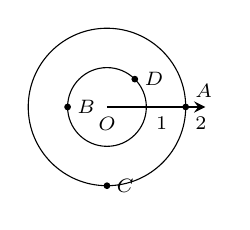
\begin{tikzpicture}[scale=.5]
\foreach \x in {1,2} {
	\draw (0,0) circle (\x);
	\draw (\x,0) node [below right] {\scriptsize $\x$};
}
\draw [thick,->,>=stealth] (0,0) node [below] {\scriptsize $O$} -- (2.5,0);
\filldraw (xyz polar cs: angle=0,radius=2) circle (2pt) node [above right] {\scriptsize $A$}
 (xyz polar cs: angle=180,radius=1)circle (2pt) node [right] {\scriptsize $B$}
 (xyz polar cs: angle=90,radius=-2)circle (2pt) node [right] {\scriptsize $C$}
 (xyz polar cs: angle=45,radius=1)circle (2pt) node [right] {\scriptsize $D$};
\end{tikzpicture}
\end{minipage}}

\exercise{Plot the points with the given polar coordinates.\\
\begin{minipage}[t]{.5\linewidth}
\begin{enumerate}
	\item $A(2,3\pi)$
	\item $B(1,-\pi)$
\end{enumerate}
\end{minipage}%
\begin{minipage}[t]{.5\linewidth}
\begin{enumerate}\addtocounter{enumii}{2}
	\item $C(1,2)$
	\item $D(1/2,5\pi/6)$
\end{enumerate}
\end{minipage}}{\mbox{}\\\begin{minipage}[m]{\linewidth}
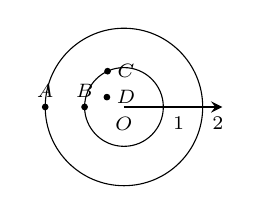
\begin{tikzpicture}[scale=.5]
\foreach \x in {1,2} {
 \draw (0,0) circle (\x);
 \draw (\x,0) node [below right] {\scriptsize $\x$};
}
\draw [thick,->,>=stealth] (0,0) node [below] {\scriptsize $O$} -- (2.5,0);
\filldraw (xyz polar cs: angle=180,radius=2) circle (2pt) node [above] {\scriptsize $A$}
 (xyz polar cs: angle=180,radius=1)circle (2pt) node [above] {\scriptsize $B$}
 (xyz polar cs: angle=114.6,radius=1)circle (2pt) node [right] {\scriptsize $C$}
 (xyz polar cs: angle=150,radius=.5)circle (2pt) node [right] {\scriptsize $D$};
\end{tikzpicture}
\end{minipage}}

\exercise{For each of the given points give two sets of polar coordinates that identify it, where $0\leq \theta\leq 2\pi$.

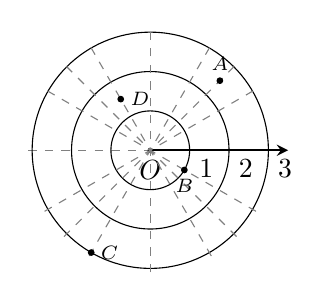
\begin{tikzpicture}[scale=.5]
	\draw [dashed,gray] (-3.1,0) -- (0,0);
	\draw[thick,->,>=stealth] (0,0) node [below] {$O$} -- (3.5,0) ;
	\filldraw (0,0) circle (1.5pt);
	\foreach \x in {1,2,3} {
		\draw (0,0) circle (\x cm);
		\draw (\x,0) node [below right] {\x};
	}
	\foreach \x in {30,45,60,90,120,135,150} {
		\draw [rotate=\x,dashed,gray] (-3.1,0) -- (3.1,0);
	}
	\filldraw (xyz polar cs: angle=45,radius=2.5) circle (2pt) node [above] {\scriptsize $A$}
		(xyz polar cs: angle=-30,radius=1)circle (2pt) node [below] {\scriptsize $B$}
		(xyz polar cs: angle=240,radius=3)circle (2pt) node [right] {\scriptsize $C$}
		(xyz polar cs: angle=120,radius=1.5)circle (2pt) node [right] {\scriptsize $D$};
\end{tikzpicture}}{$A(2.5,\pi/4)$ and $A(-2.5,5\pi/4)$;\\
$B(-1,5\pi/6)$ and $B(1,11\pi/6)$;\\
$C(3,4\pi/3)$ and $C(-3,\pi/3)$;\\
$D(1.5,2\pi/3)$ and $D(-1.5,5\pi/3)$}

\exercise{For each of the given points give two sets of polar coordinates that identify it, where $-\pi\leq \theta\leq \pi$.

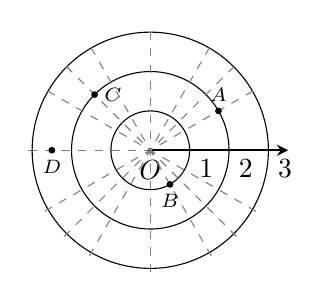
\begin{tikzpicture}[scale=.5]
	\draw [dashed,gray] (-3.1,0) -- (0,0);
	\draw[thick,->,>=stealth] (0,0) node [below] {$O$} -- (3.5,0) ;
	\filldraw (0,0) circle (1.5pt);
	\foreach \x in {1,2,3}
	{\draw (0,0) circle (\x cm);
	\draw (\x,0) node [below right] {\x};
	}
	\foreach \x in {30,45,60,90,120,135,150}
	{\draw [rotate=\x,dashed,gray] (-3.1,0) -- (3.1,0);
	}
	\filldraw (xyz polar cs: angle=30,radius=2) circle (2pt) node [above] {\scriptsize $A$}
	      (xyz polar cs: angle=-60,radius=1)circle (2pt) node [below] {\scriptsize $B$}
				(xyz polar cs: angle=135,radius=2)circle (2pt) node [right] {\scriptsize $C$}
				(xyz polar cs: angle=180,radius=2.5)circle (2pt) node [below] {\scriptsize $D$};
	
\end{tikzpicture}	
}{$A(2,\pi/6)$ and $A(-2,-5\pi/6)$;\\
$B(1,-\pi/3)$ and $B(-1,2\pi/3)$;\\
$C(2,3\pi/4)$ and $C(-2,-\pi/4)$;\\
$D(2.5,\pi)$ and $D(2.5,-\pi)$}

\exercise{Convert the polar coordinates A and B to rectangular, and the rectangular coordinates C and D to polar.\\
\begin{minipage}[t]{.5\linewidth}
\begin{enumerate}
	\item $A(2,\pi/4)$
	\item $B(2,-\pi/4)$
\end{enumerate}
\end{minipage}%
\begin{minipage}[t]{.5\linewidth}
\begin{enumerate}\addtocounter{enumii}{2}
	\item $C(2,-1)$
	\item $D(-2,1)$
\end{enumerate}
\end{minipage}
}{$A=(\sqrt{2},\sqrt{2})$;\\
$B=(\sqrt{2},-\sqrt{2})$;\\
$C=(\sqrt{5},-0.46)$;\\
$D=(\sqrt{5},2.68)$}

\exercise{Convert the polar coordinates A and B to rectangular, and the rectangular coordinates C and D to polar.\\
\begin{minipage}[t]{.5\linewidth}
\begin{enumerate}
	\item $A(3,\pi)$
	\item $B(1,2\pi/3)$
\end{enumerate}
\end{minipage}%
\begin{minipage}[t]{.5\linewidth}
\begin{enumerate}\addtocounter{enumii}{2}
	\item $C(0,4)$
	\item $D(1,-\sqrt{3})$
\end{enumerate}
\end{minipage}
}{$A=(-3,0)$;\\
$B=(-1/2,\sqrt{3}/2)$;\\
$C=(4,\pi/2)$;\\
$D=(2,-\pi/3)$}

\input{exercises/09-04-exset-01}

\input{exercises/09-04-exset-02}

\begin{exerciseset}{In Exercises}{, convert the  rectangular equation to a polar equation.}

\exercise{$\ds y=x$}{$\theta=\pi/4$}

\exercise{$\ds y=4x+7$}{$r=7/(\sin\theta-4\cos\theta)$}

\exercise{$\ds x=5$}{$r=5\sec \theta$}

\exercise{$\ds y=5$}{$r=5\csc \theta$}

\exercise{$\ds x=y^2$}{$r=\cos\theta/\sin^2\theta$}

\exercise{$\ds x^2y=1$}{$r=1/\sqrt[3]{\cos^2\theta\sin\theta}$}

\exercise{$\ds x^2+y^2=7$}{$r=\sqrt{7}$}

\exercise{$\ds (x+1)^2+y^2=1$}{$r=-2\cos\theta$}

\end{exerciseset}


\input{exercises/09-04-exset-04}

\exercise{Pick a integer value for $n$, where $n\neq 2,3$, and use technology to plot $\ds r=\sin\left(\frac mn\theta\right)$ for three different integer values of $m$. Sketch these and determine a minimal interval on which the entire graph is shown.}{Answers will vary. If $m$ and $n$ do not have any common factors, then an interval of $2n\pi$ is needed to sketch the entire graph.
}

\exercise{Create your own polar function, $r=f(\theta)$ and sketch it. Describe why the graph looks as it does.}{Answers will vary.
}
